\chapter{System Design}
In this chapter, I will be discussing the overall design of the levels and UI elements in the game along with going through all the C\# scripts that I used in the game.I will show code snippets and game screenshots to explain the design of the project and how everything works. I will be breaking this chapter into three parts, Level design, coding and the final build, Firstly for the level design, I will be showing screenshots of early design ideas and why i chose not to include some of the early ideas. I will then look at the  c\# scripts used to make the game function and how Unity uses the scripts. Lastly i will be showing screenshots and giving descriptions of each on what the final build looks like. The final build will be what the users will be interacting with in order to play the game.

\section{Game Design}
In this section I will be discussing the early stage development designs for the levels and the final level designs used. Also included is the characters and scenes that never made it into the final builds as well as reasons for not including them, along with the final character designs.

\subsection{Early Designs}
During the early stages of development, I had several ideas for the game which in the end never made it into final production. These included level designs, character designs, character selection screens and different menu layouts. The reason for these not making the final product was due to either me coming up with a better idea than them or feeling that I did not want to include them in the final build. Below are all shots of the sketches of early level designs, character designs as well as a concept for a character selection screen.

\begin{figure}
\centering
\begin{subfigure}{.5\textwidth}
\centering
  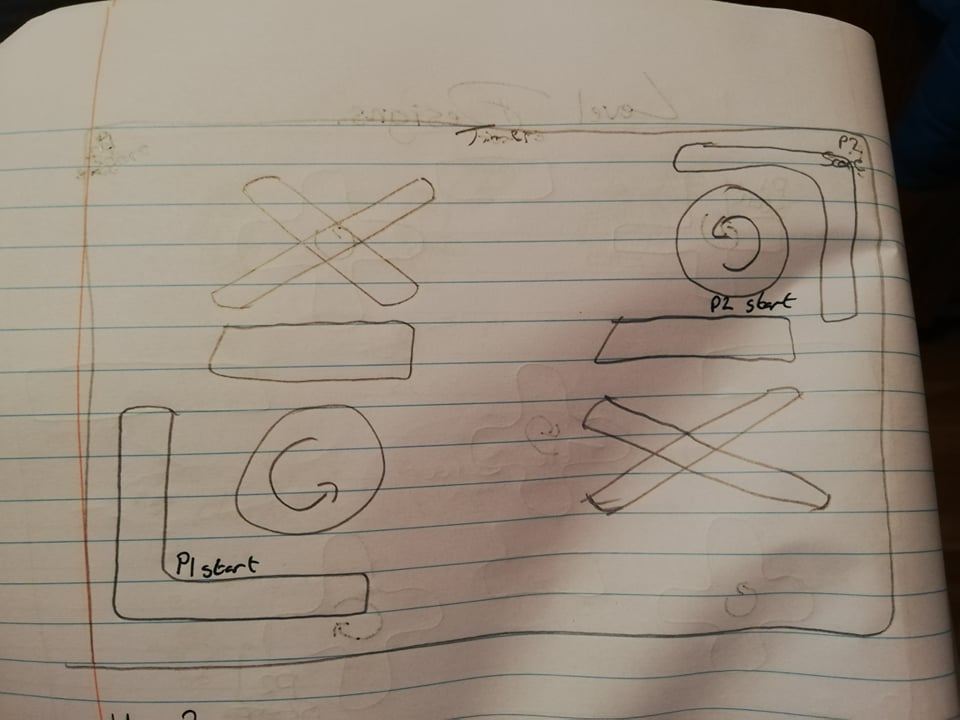
\includegraphics[width= 1\linewidth]{Images/Leveldesign1.jpg}
  \caption{Level Concept 1.}
  \label{fig:Level1 Concept}
\end{subfigure}%
\begin{subfigure}{.5\textwidth}
\centering
  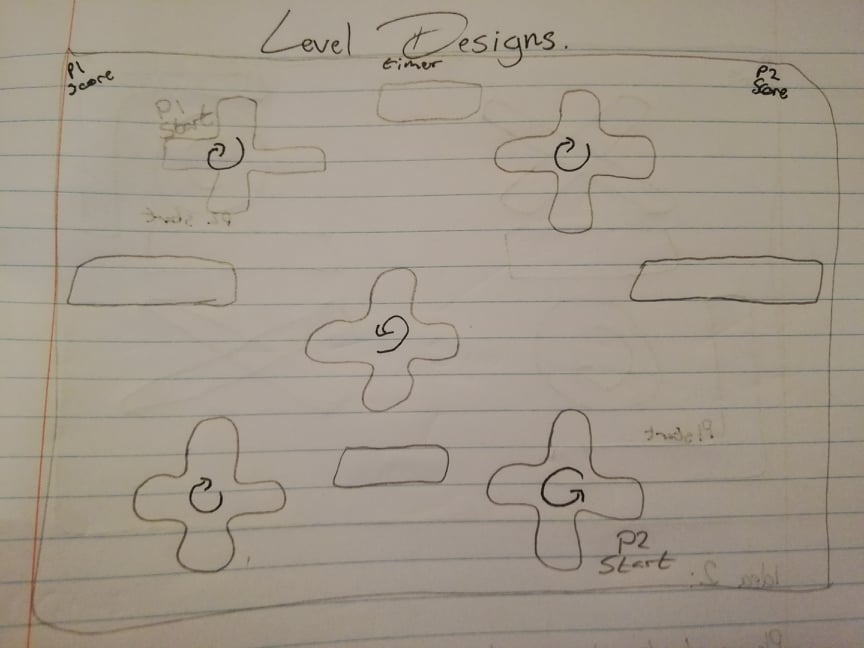
\includegraphics[width= 1\linewidth]{Images/Leveldesign2.jpg}
  \caption{Level Concept 2.}
  \label{fig:Level2 Concept}
  \end{subfigure}%
  \newline
\begin{subfigure}{.5\textwidth}
\centering
  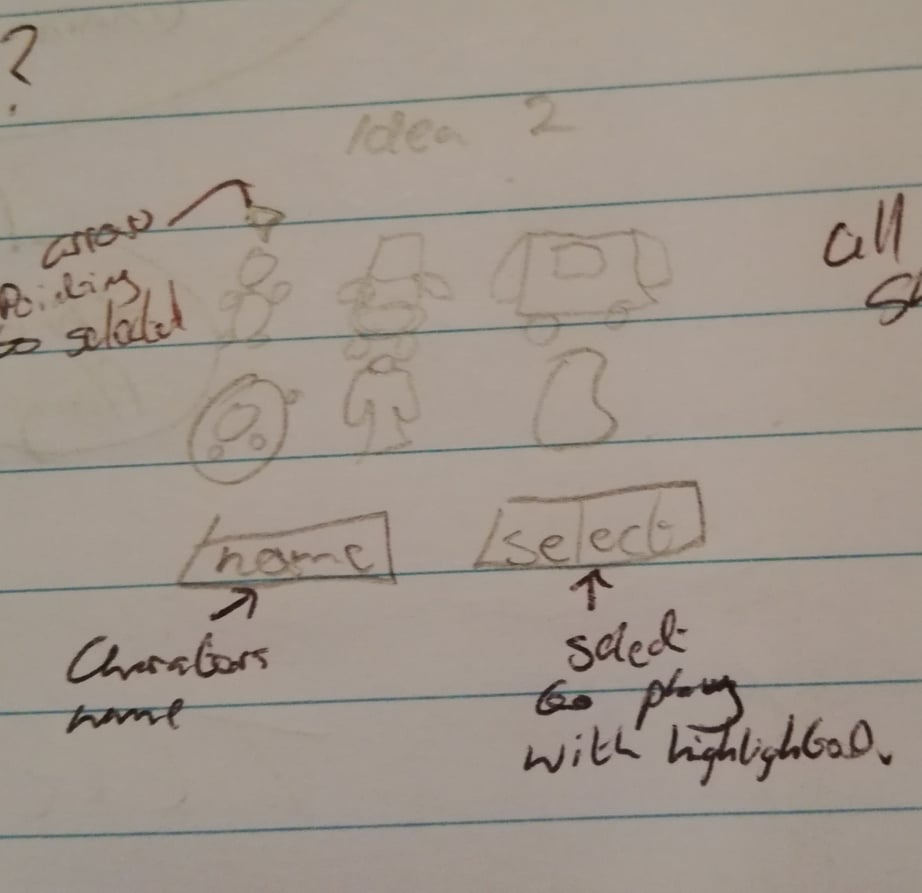
\includegraphics[width= 1\linewidth]{Images/CharacterSelectionIdea.jpg}
  \caption{Character Selection Idea 1.}
  \label{fig:CharacterSelectionIdea}
  \end{subfigure}%
\begin{subfigure}{.5\textwidth}
\centering
  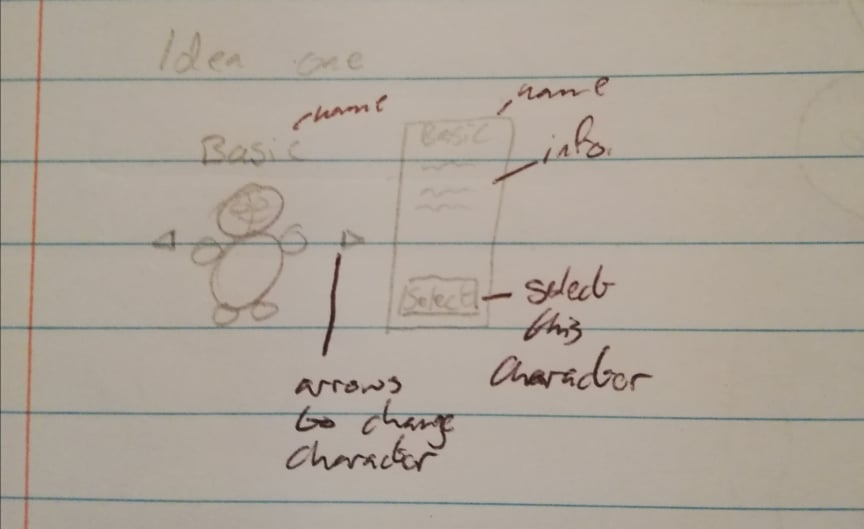
\includegraphics[width= 1\linewidth]{Images/CharacterSelectionIdea2.jpg}
  \caption{Character Selection Idea 2.}
  \label{fig:CharacterSelectionIdea2}
  \end{subfigure}%
  \newline
\begin{subfigure}{.5\textwidth}
\centering
  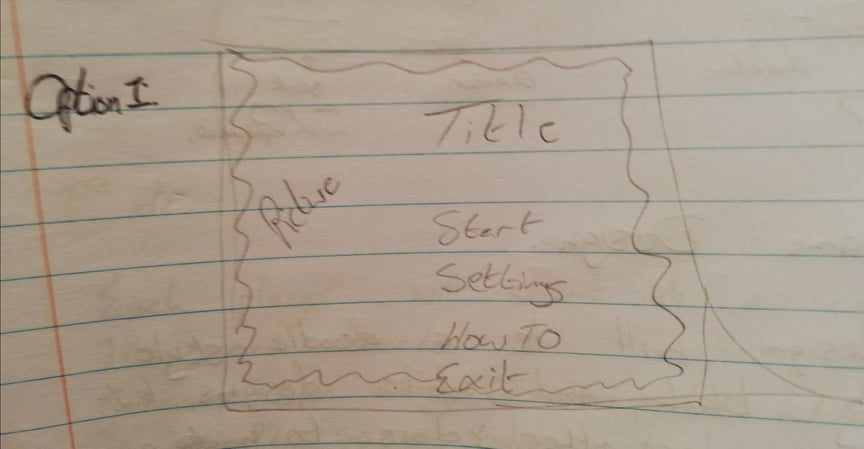
\includegraphics[width= 1\linewidth]{Images/MenuIdea.jpg}
  \caption{Menu Idea 1.}
  \label{fig:MenuIdea1}
  \end{subfigure}%
\begin{subfigure}{.5\textwidth}
\centering
  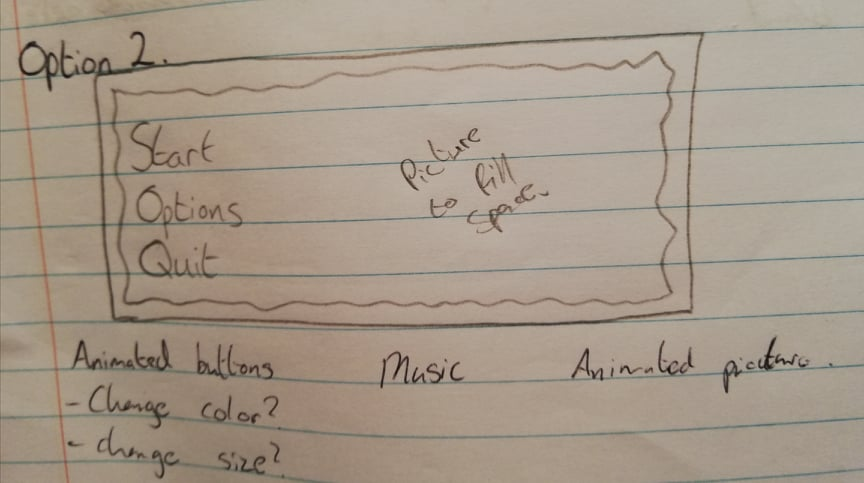
\includegraphics[width= 1\linewidth]{Images/MenuIdea2.jpg}
  \caption{Menu Idea 2.}
  \label{fig:MenuIdea2}
  \end{subfigure}%
\end{figure}

\newpage
Originally I had planned on doing a character selection screen for my game, see figure \ref{fig:CharacterSelectionIdea} and figure \ref{fig:CharacterSelectionIdea2} where you could choose to use different types of characters that would have variant types of boosts like better speed, stronger hits and higher jumps but after researching on it I came to the conclusion that because of the level designs it would run the risk of having overpowered characters like the higher jump character being able to escape the other character too quickly making it very difficult for the other player to shoot him. In the end I decided to take this idea out of the game altogether to allow for an even playing field of just two characters that boast the same stats in terms of speed, jumping and shot power.

\section{Menu Designs}
\begin{figure}[h]
\centering
  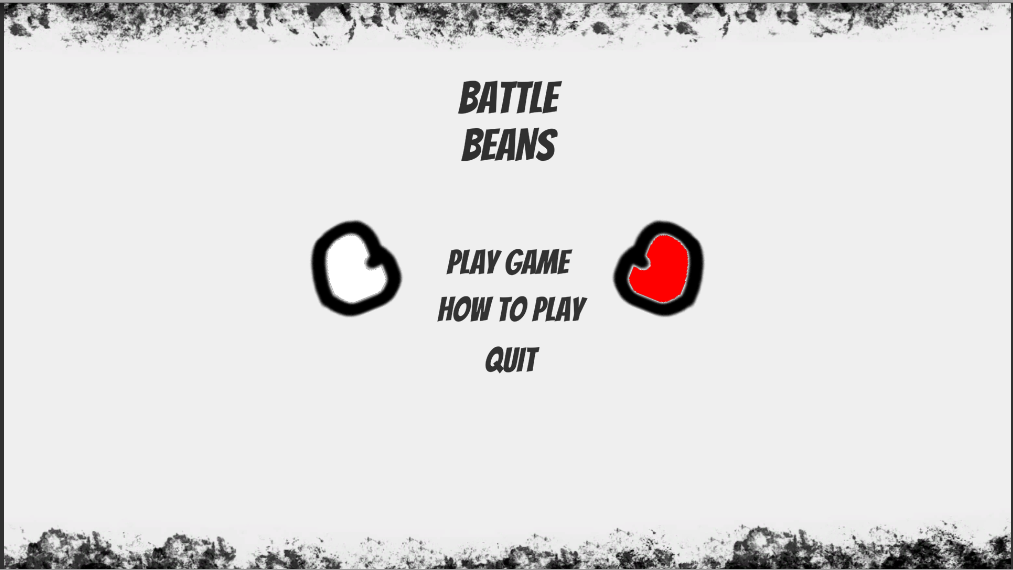
\includegraphics[width= 0.8\linewidth]{Images/MainMenu.PNG}
  \caption{Main Menu.}
  \label{fig:Menu}
\end{figure}

In this section I will be going through the design for the main menu at the start of the game showing how each element of it worked and how it looked during game play. To start, I created a canvas and called it MainMenu. This menu consisted of a text box for the title, three selectable buttons to play the game, to learn about the game and a button to allow the user to exit the application. 

\begin{figure}[h]
\centering
\begin{subfigure}{.5\textwidth}
\centering
  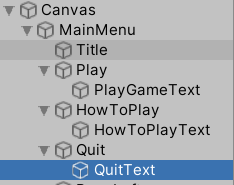
\includegraphics[width= 0.5\linewidth]{Images/MainMenuElements.PNG}
  \caption{Menu Elements.}
  \label{fig:MenuEle}
  \end{subfigure}%
  \begin{subfigure}{.5\textwidth}
\centering
  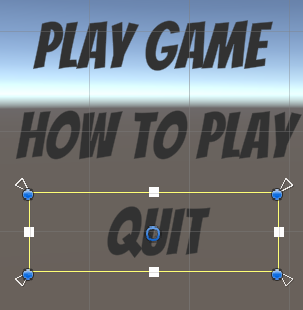
\includegraphics[width= 0.5\linewidth]{Images/TextBox.PNG}
  \caption{Quit Text Box in Yellow.}
  \label{fig:TextBox}
  \end{subfigure}%
\end{figure}
\newpage

\begin{figure}[h]
\centering
  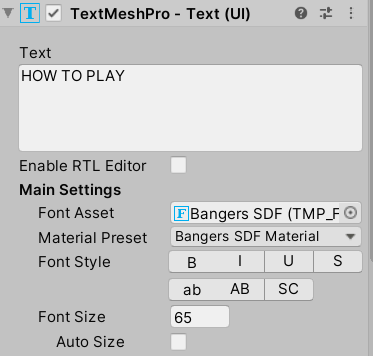
\includegraphics[width= 0.8\linewidth]{Images/TextEditor.PNG}
  \caption{Text Editor Example.}
  \label{fig:Text Editor}
\end{figure}

Each of the text boxes are children of a button function in which when pressed would lead to a new UI element. This is done by creating an on click function in the button field in the inspector, see figure \ref{fig:OnClick()}, where you would drag in the UI element you want and add a set active function to turn a UI element on or off by ticking a box. For example, if you click on the Play Game button, the Main Menu UI will be turned off and the Level Select UI will be turned on, allowing the player to see a new level select menu.
\begin{figure}[h]
\centering
  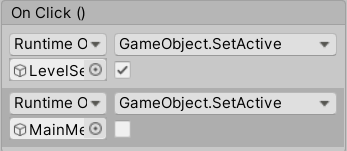
\includegraphics[width= 0.8\linewidth]{Images/OnClick.PNG}
  \caption{OnClick() function.}
  \label{fig:OnClick()}
\end{figure}
This is done for each different UI screen so that you can switch between them on the clicking the buttons so that there is no overlap of different UI's. For the Level Select UI however, in order for the buttons to be bring you to the different level scenes a script is needed in order to actually load the level scene you want to play. For this you would drag in the UI element that holds the script that is used to load the levels and set which method in the script you want to run that will load the desired scene. Below is a code snippet of the code required in order to load a level.
\begin{figure}[h]
\centering
  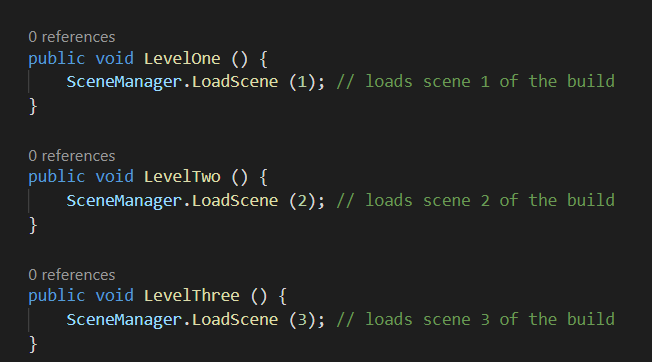
\includegraphics[width= 0.8\linewidth]{Images/LevelSelectCode.PNG}
  \caption{Code Snippet from MainMenu.}
  \label{fig:Level}
\end{figure}

\newpage
The same can be done for the the quit button on the main menu where the method for quitting the game is called which closes the application when being ran from the built version of the game. The code snippet below shows how this is done along with an extra line called Debug.log() which is used to test that the feature works when working from inside Unity through the console as when it is pressed while running the game in the game window, it wont actually exit the game as the application has not actually been made.

\begin{figure}[h]
\centering
\begin{subfigure}{.5\textwidth}
\centering
  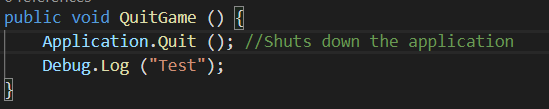
\includegraphics[width= 0.8\linewidth]{Images/Quit.PNG}
  \caption{Code Snippet for Quit();.}
  \label{fig:Quit}
  \end{subfigure}%
  \begin{subfigure}{.5\textwidth}
\centering
  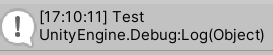
\includegraphics[width= 0.8\linewidth]{Images/QuitTest.PNG}
  \caption{Testing Quit in the console.}
  \label{fig:Debug}
  \end{subfigure}%
\end{figure}
\subsection{Final Menu View}
This subsection will be used to show how each menu UI turned out in the final build of the game.

\begin{figure}[h]
\centering
\begin{subfigure}{.5\textwidth}
\centering
  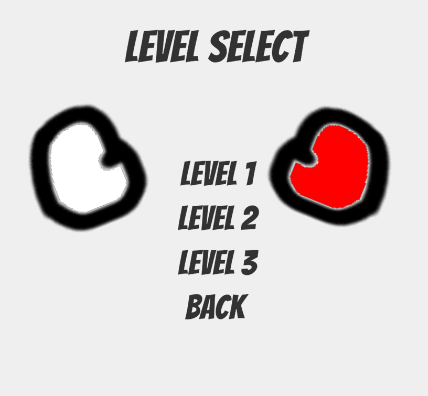
\includegraphics[width= 0.8\linewidth]{Images/LevelSelect.PNG}
  \caption{Level Select Menu.}
  \label{fig:LevelSelectMenu}
  \end{subfigure}%
  \begin{subfigure}{.5\textwidth}
\centering
  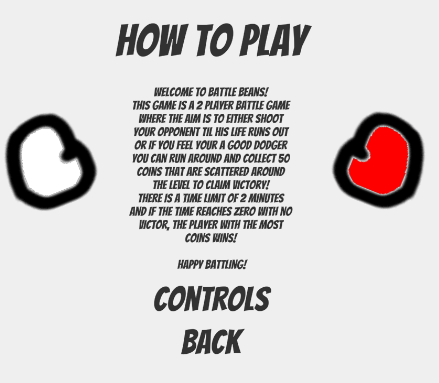
\includegraphics[width= 0.8\linewidth]{Images/How To Play.PNG}
  \caption{How To Play Menu.}
  \label{fig:HTP}
  \end{subfigure}%
  \newline
    \begin{subfigure}{.5\textwidth}
\centering
  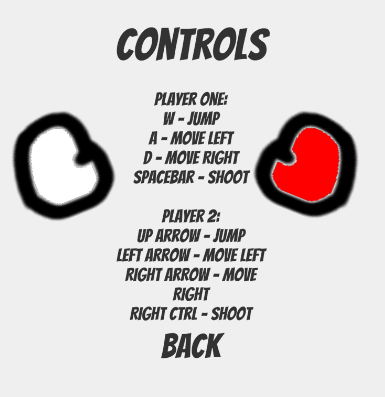
\includegraphics[width= 0.8\linewidth]{Images/Controls.PNG}
  \caption{Controls Menu.}
  \label{fig:Controls}
  \end{subfigure}%
\end{figure}
\newpage

\section{Level Design}
In this section I will go through the design of each of the three levels present in the final build of the game. I will be showing shots of the final build of the levels and how it was made as well as the sprites used to create the platforms, the items that can be picked up and how spawn points were made for coins and health.

\subsection{Sprites}
For the design of the levels, I put in simple sprites that I made using the image editor GIMP and how I added colliders and scripts to them so that they would provide functionality to the game. These will include how I made health items so that the players can regain their health, coin items so that a score could be gained from collecting them, the animations used and how I added colliders platforms and borders so that the players could not go through them.

\subsection{Environment Sprites}
As stated above, I used the image editing software GIMP, described in section 3.3.1, to create the sprites needed for the levels layouts. Once the images were created in GIMP, they were exported to PNG images for use in Unity. Once they were in Unity, a folder was created and named Sprites so that I could easily sort and find all the sprite images needed for development. To use the sprites, I simply clicked and dragged them into the scene view in Unity which would place them in the scene I was working on. Once they were added to the scene, I would add either a Box Collider 2D component or a Circle Collider which would put either an invisible box or circle around the sprite image so that the player character would not simply just slip through it and fall out of the level. The collider would then show a green outline to show the size of the collider added which could be edited by pressing the Edit Collider button in the inspector, see figure below, \ref{fig:Green} and \ref{fig:ColliderMenu}.
\begin{figure}[h]
\centering
  \begin{subfigure}{.5\textwidth}
\centering
  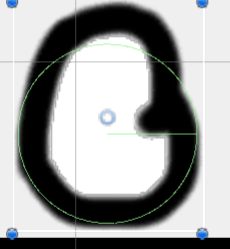
\includegraphics[width= 0.5\linewidth]{Images/ColliderOnObject.PNG}
  \caption{Example of green outline on Sprite.}
  \label{fig:Green}
  \end{subfigure}%
    \begin{subfigure}{.5\textwidth}
\centering
  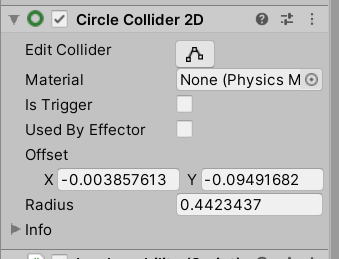
\includegraphics[width= 0.8\linewidth]{Images/ColliderInspector.PNG}
  \caption{Collider menu in Inspector.}
  \label{fig:ColliderMenu}
  \end{subfigure}%
\end{figure}
\newpage

For the levels platforms, as well as adding a box collider to them so that the player could stand on them without falling through, I added a feature that would allow the player to jump through the bottom of the platform allowing for easy access to collect the coins that would appear and allow the player to quickly escape the other player without getting trapped. I did this by adding a component called "Platform Effector 2D" which would allow you to create a surface arc of 180 degree and setting it to one way allowing the player to jump through the bottom but not slip through the top. Once this was added, a tick box would be selected in the box/circle collider to allow it to use the effector component which would enable it to work.

\begin{figure}[h]
\centering
  \begin{subfigure}{.5\textwidth}
\centering
  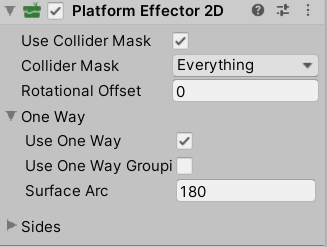
\includegraphics[width= 0.8\linewidth]{Images/PlatformEffector2D.PNG}
  \caption{Platform Effector.}
  \label{fig:PlatEffect}
  \end{subfigure}%
    \begin{subfigure}{.5\textwidth}
\centering
  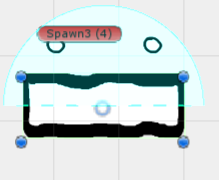
\includegraphics[width= 0.8\linewidth]{Images/PlatformWithEffector.PNG}
  \caption{Platform with effector on.}
  \label{fig:PlatEffOn}
  \end{subfigure}%
\end{figure}

\subsection{Using Scripts On Sprites}
For a couple of sprites, Scripts had to be added to provide functionality to them. These include the coins used to add up the players score, health items so that the player could regain lost health and a script to add functionality to the player sprite so that it could move, jump, shoot, take damage, etc. 

\subsection{Coins}

\begin{figure}[h]
\centering
  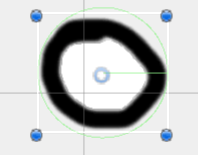
\includegraphics[width= 0.3\linewidth]{Images/Coin.PNG}
  \caption{Coin Sprite.}
  \label{fig:Coin}
\end{figure}

For the coins, I added a circle collider and set "Is Trigger" to be on as for the script I needed the collider to be a trigger so that when the players collider hit the coins collider it would register that the colliders had hit each other so that the method OnTriggerEnter2D in the Coin script could run, see Figure \ref{fig:CoinTrig}.

\begin{figure}[h]
\centering
  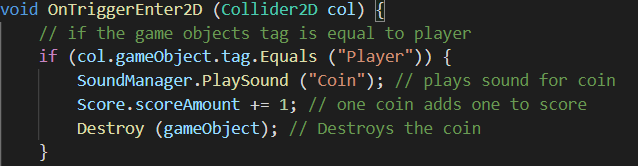
\includegraphics[width= 0.8\linewidth]{Images/CoinTrigger.PNG}
  \caption{Code Snippet from Coin.}
  \label{fig:CoinTrig}
\end{figure}

For this the coin would only react to a gameObject that contained the tag "Player", which is the tag given to the player gameObject. Once the coin recognized that it was the player that hit it, it would then add a value of 1 to the players score vale, more on this later, and then destroy itself so that it cant be continuously picked up with out actually disappearing, see figure \ref{fig:Health}.

\subsection{Health}
\begin{figure}[h]
\centering
  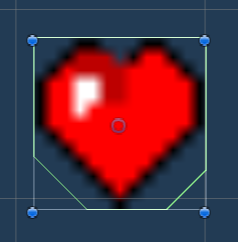
\includegraphics[width= 0.2\linewidth]{Images/Heart.PNG}
  \caption{Heart Sprite.}
  \label{fig:Heart}
\end{figure}
For the Heart and health, I added a Polygon Collider to it as this fits the sprite image itself, which is useful for sprites that are not circular or square, and also set this to have "Is Trigger" set to on similarly to the coin sprite. Like the coin sprite, the heart sprite also had a OnTriggerEnter2D method so that it could run when the the player game object with the tag "Player" collided with it.
\begin{figure}[h]
\centering
  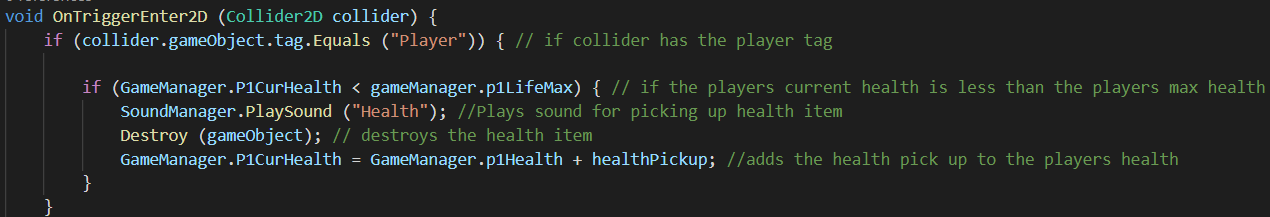
\includegraphics[width= 1\linewidth]{Images/HealthTrigger.PNG}
  \caption{Code snippet from HealthPickUp.}
  \label{fig:Health}
\end{figure}
\newline
Similarly to the coin script, when the player hit the heart sprite if the players health was lower than it's max health, it would add 1 health to the players current health but not if the player was already at max health. It would then destroy itself so that it couldn't be continuously picked up.


\subsection{Player}
\begin{figure}[h]
\centering
  
\includegraphics[width= 0.3\linewidth]{Images/Player.PNG}
  \caption{Player Sprite.}
  \label{fig:Player}
\end{figure}
For each player, a circle collider was added and a PlayerController script was attached to them to allow functionality to the player. Variables were made for moving left, moving right, jumping, shooting, movement speed and jump force. These variables could be set for each player by assigning them to buttons using the fields in the Inspector view, see figure \ref{fig:PlayerInspect}. Along with adding these variables, there was more added to let Unity know which prefab was being used to act as the projectile used as the bullet for shooting and a field to set what was considered the ground for the player.

\begin{figure}[h]
\centering
  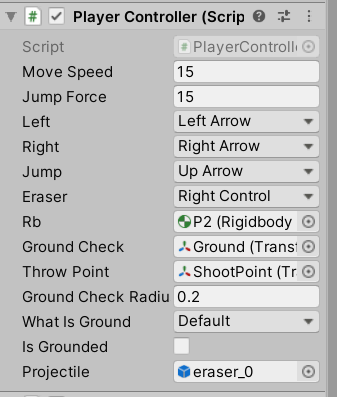
\includegraphics[width= 0.4\linewidth]{Images/PlayerControllerInspector.PNG}
  \caption{PlayerController Inspector view.}
  \label{fig:PlayerInspect}
  \end{figure}
\begin{figure}[h]
\centering
  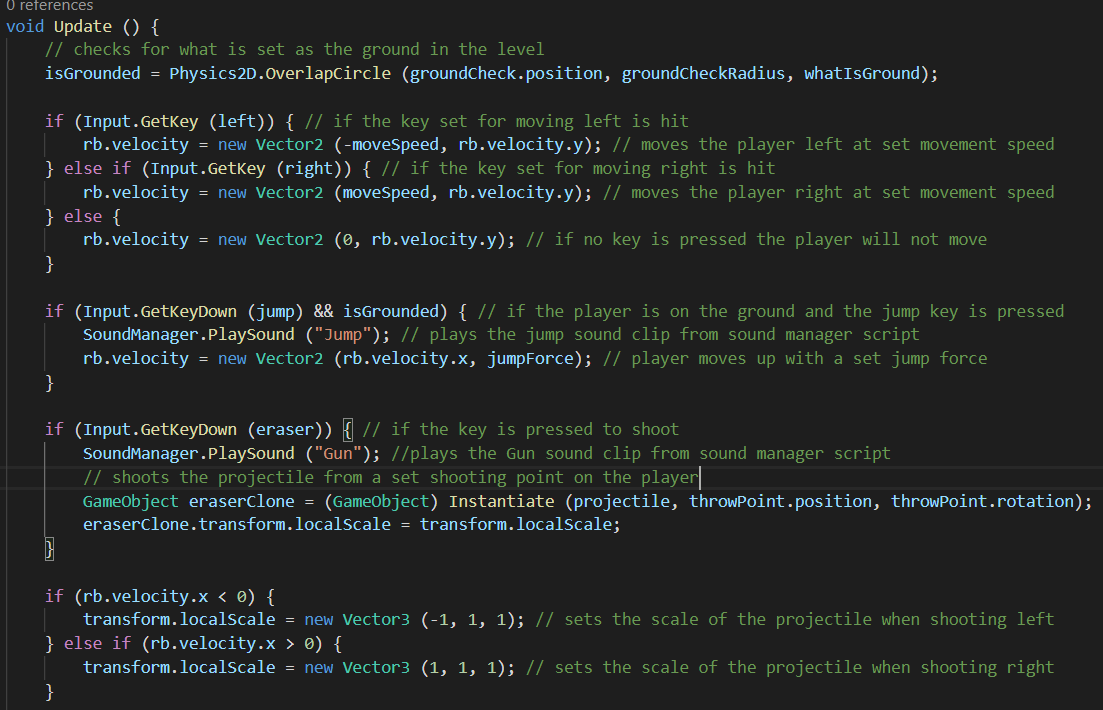
\includegraphics[width= 0.9\linewidth]{Images/PlayerController.PNG}
  \caption{Code Snippet From PlayerController.}
  \label{fig:PlayerControllerCode}
\end{figure}

Another script that was added to the player was the Invulnerability script which made it possible for the bullets to go straight through the player after being hit for 2 seconds. The reason this script was added was so that it gave the player a chance to get away from being attacked by the other player so that they wouldn't get spam shot meaning they would die very quickly. This was done by making the projectile layer ignore the player layer when the player was hit, making a transparent effect on the player for two seconds. It also meant that the player couldn't damage the other player while they were in the Invulnerable state as that would be unfair. See figure \ref{fig:Invulnerable}

\begin{figure}[h]
\centering
  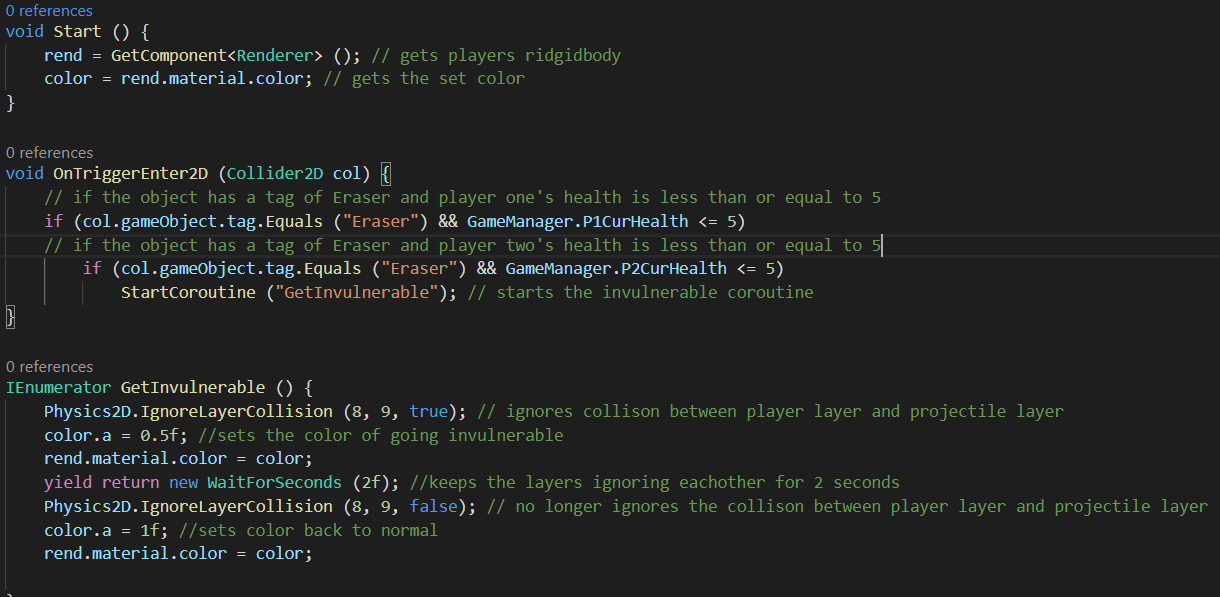
\includegraphics[width= 0.9\linewidth]{Images/Invulnerable.PNG}
  \caption{Code Snippet From Invulnerable.}
  \label{fig:Invulnerable}
\end{figure}
\newpage

\section{Game Manager}
The GameManager script was the biggest script involved in making the game as it contained ways for the players health to display as full and empty heart sprites to determine how much health a player had, how the player took damage, how to determine which winning screen it would show (Player one win screen or player two) and to be able to pause the game. This section will be used to describe how each of those mentioned above.

\subsection{Player Health System}
For the games health system, I decided to use a heart system similar to that in the Legend of Zelda games where a full heart represents 1 health and an empty heart represents health lost. To do this I set up two image arrays, one for a player one's hearts and one for player two's hearts. Then, using a for loop, I determined if the players health was less than the number of hearts. The number of hearts was set to be equal to the players health, so if one health was taken away it would mean that one full heart would be taken away and replace with an empty heart, see figure \ref{fig:Hearts}. I also set it so that the player can only have a number of 5 hearts in the inspector by setting max life to 5.
\begin{figure}[h]
\centering
  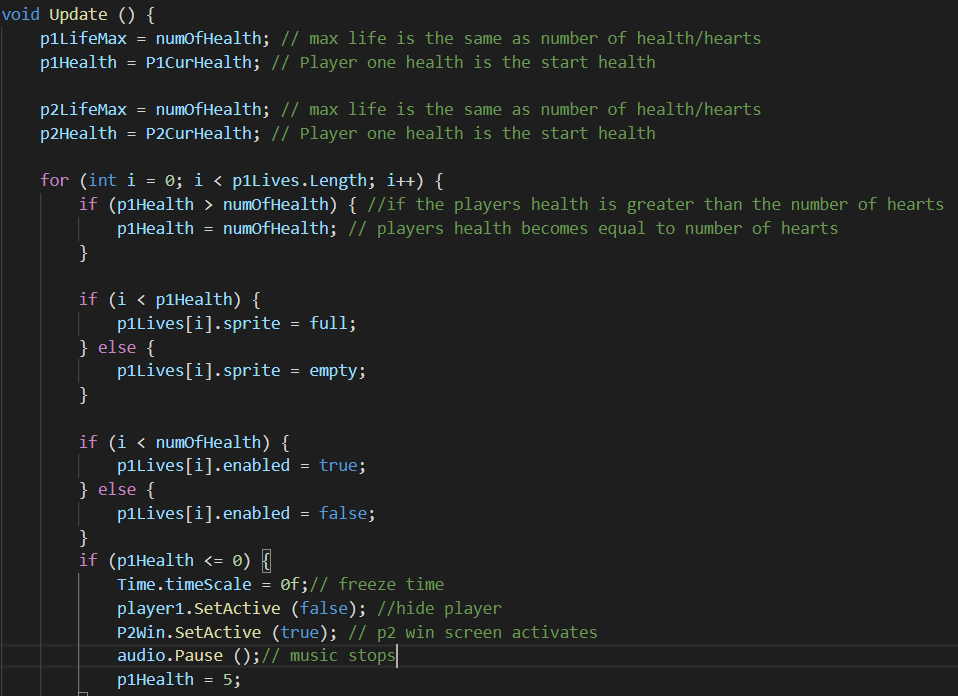
\includegraphics[width= 0.9\linewidth]{Images/HealthSystem.PNG}
  \caption{Code Snippet From GameManager.}
  \label{fig:GameManagerCode}
\end{figure}
\begin{figure}
\begin{subfigure}{.4\textwidth}
\centering
  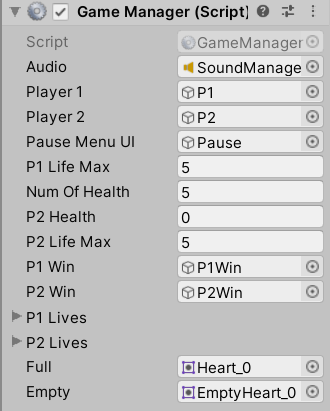
\includegraphics[width= 1\linewidth]{Images/GameManagerInspect.PNG}
  \caption{GameManager in the inspector.}
  \label{fig:GameManager}
  \end{subfigure}
  \begin{subfigure}{.5\textwidth}
\centering
  
\includegraphics[width= 1\linewidth]{Images/Hearts.PNG}
  \caption{Hearts Health system.}
  \label{fig:Hearts}
  \end{subfigure}
\end{figure}
\newpage

\subsection{UI Elements}
In this section I will be explaining how each of the player win screens, the pause screen, the draw screen, the score display and the timer display worked. Firstly for the the player wins screens, I added them very similarly to how I added all the elements to to the main menu UI in terms of adding text boxes to display "Player 1/2 Wins!!" and the buttons to go back to the main menu, seen in section 4.2. The main difference was that I had to add a snippet of code into the game manager to make the player win UI appear when a player brought the other players health down to zero. I also the same snippet of code to both the score scripts for when the players reached 50 points and for  the Countdown script so winner could be determined after the timer had reached 0. For when a players health reached zero, I made it so that when a players health would reach zero it would freeze the game using Time.timeScale function by setting it to 0. Then I would set the Player win UI element to active so that it would appear after either player one's or player two's health was equal to zero, as it is default set to be inactive. Below is a shot of the code snippet used to make this possible.

\begin{figure}[h]
\centering
  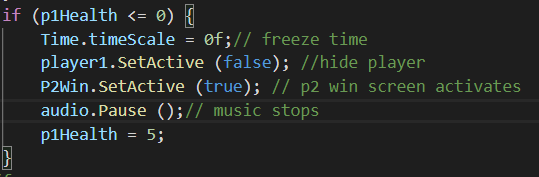
\includegraphics[width= 0.7\linewidth]{Images/P2Wins.PNG}
  \caption{Code Snippet For if player 2 wins.}
  \label{fig:P2Win}
\end{figure}

Similarly for both when a player reaches a score of 50 and determining a winner after the timer reaches 0, I wrote code for it to display the UI for each player winning as well as if the players had the same score after the timer finishes it would display a screen saying that the game had finished in a draw, with a button that on click would bring you back to the main menu. See below for code snippets of both Winning with score and getting the draw screen as well as determining a winner if the timer reaches 0.

\begin{figure}[h]
\begin{subfigure}{1\textwidth}
\centering
  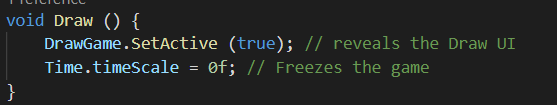
\includegraphics[width= 1\linewidth]{Images/Draw.PNG}
  \caption{Code Snippet for Draw.}
  \label{fig:Draw}
  \end{subfigure}
  \newline
  \begin{subfigure}{1\textwidth}
\centering
  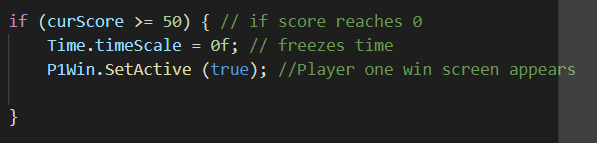
\includegraphics[width= 1\linewidth]{Images/ScoreWinner.PNG}
  \caption{Code snippet for win at 50.}
  \label{fig:scorewin}
  \end{subfigure}
  \newline
    \begin{subfigure}{1\textwidth}
\centering
  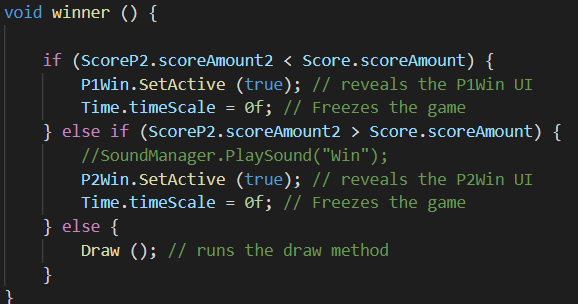
\includegraphics[width = 1\linewidth]{Images/ScoreWinnersCountdown.PNG}
  \caption{Code snippet for a winner after timer hits 0}
  \label{fig:countdown}
  \end{subfigure}
\end{figure}

In order to bring up a pause screen, in the game manager I added a Boolean if the gameIsPaused is true or false and if it is true when to escape key is pressed it will display the pause menu. If the escape button is pressed again while in the pause menu, the Boolean will be returned to false and the pause menu will then become inactive, thus disappearing. Below is a snippet of code that enables the pause menu to appear along with how the pause menu looks.

\begin{figure}[h]
\begin{subfigure}{1\textwidth}
\centering
  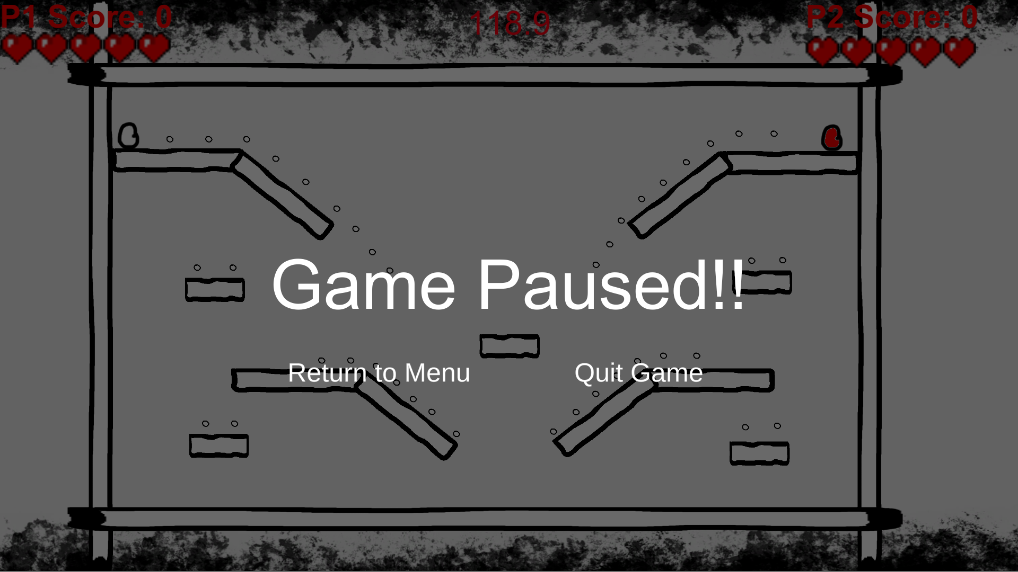
\includegraphics[width= .4\linewidth]{Images/PauseMenu.PNG}
  \caption{Pause Menu UI.}
  \label{fig:PauseUI}
  \end{subfigure}
  \begin{subfigure}{1\textwidth}
\centering
  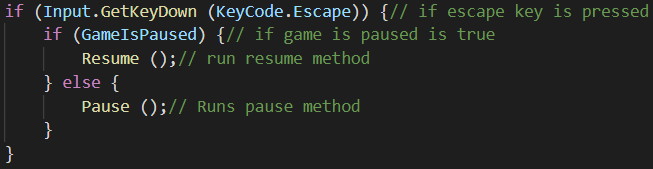
\includegraphics[width= 1\linewidth]{Images/PauseKey.PNG}
  \caption{Code snippet for Pause key.}
  \label{fig:escape}
  \end{subfigure}
  \newline
    \begin{subfigure}{1\textwidth}
\centering
  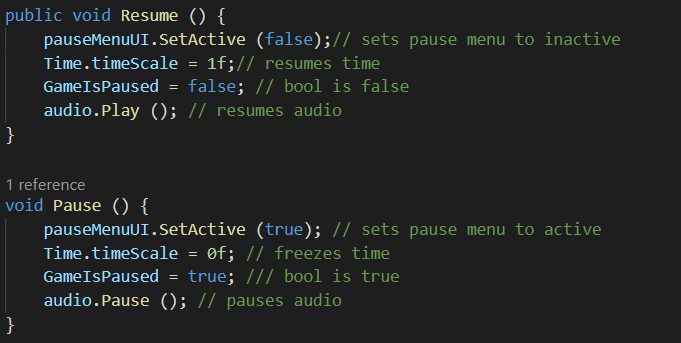
\includegraphics[width = 1\linewidth]{Images/Pause.PNG}
  \caption{Code snippet for pause methods}
  \label{fig:pause}
  \end{subfigure}
\end{figure}


For the timer, I added a text box to the middle top that displayed "0" and added a script to the canvas called Countdown. In this script I set variables for the Timer text, the current time and the start time. In the script I set the current time to be equal to the start time and in the Update() method i set the time to go down by one second every second until the timer had reached 0. once the timer had reached zero, I then set the current time to be zero so that it would stay at zero and then ran the winner method mentioned above for determining a winner based on score. Below is a snippet of code that shows how the timer works.
\begin{figure}[h]
\centering
  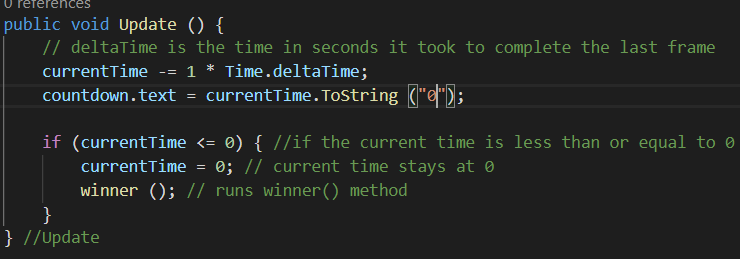
\includegraphics[width= 1\linewidth]{Images/Timer.PNG}
  \caption{Code Snippet For the timer.}
  \label{fig:Timer}
\end{figure}

\section{Spawning}
In this section I will briefly describe how I added spawnpoints for both the health items and the coins. To do this, I created two empty game objects called CoinSpawner and HealthSpawner and made children of both of these named spawn points. I then scattered the spawn points across each level and began writing a script for both the CoinSpawner and HealthSpawner. In these scripts I created arrays for both the spawnPoints and the items that will spawn at these points. Then I put an InvokeRepeating function in the start() method so that it would spawn the items at intervals of the given seconds, see figure \ref{fig:HealthSpawn} and \ref{fig:CoinSpawn}.A SpawnHealth/SpawnCoin method is then made to make the items spawn at the previously made spawn points at random. After the scripts where made, I dragged in the spawn points and the items into the correct fields displayed in the inspector, see figure \ref{fig:CoinSpawnInspect} and \ref{fig:HealthSpawnInspect}.

\begin{figure}[h]
\centering
  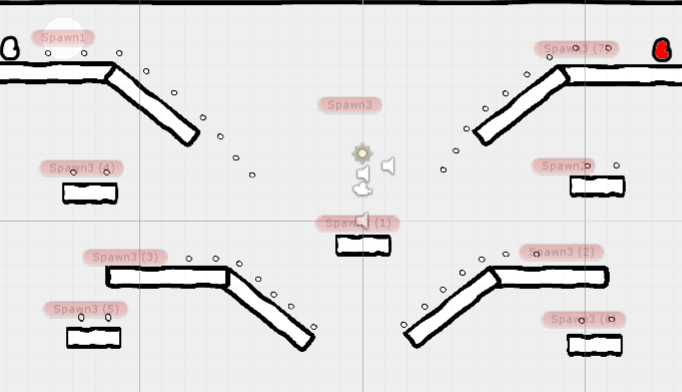
\includegraphics[width= .8\linewidth]{Images/SpawnPoints.PNG}
  \caption{Spawn Points on level in red.}
  \label{fig:SpawnPoints}
  \end{figure}

  \begin{figure}[h]
  \begin{subfigure}{1\textwidth}
\centering
  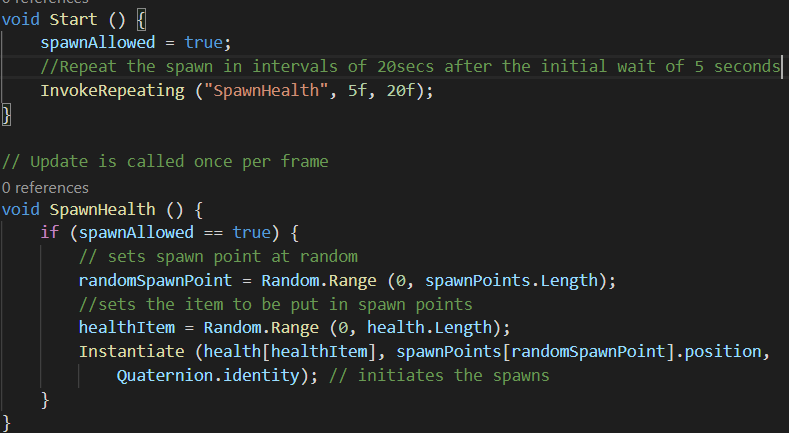
\includegraphics[width= 1\linewidth]{Images/HealthSpawn.PNG}
  \caption{Code snippet for HealthSpawn.}
  \label{fig:HealthSpawn}
  \end{subfigure}
  \begin{subfigure}{1\textwidth}
\centering
  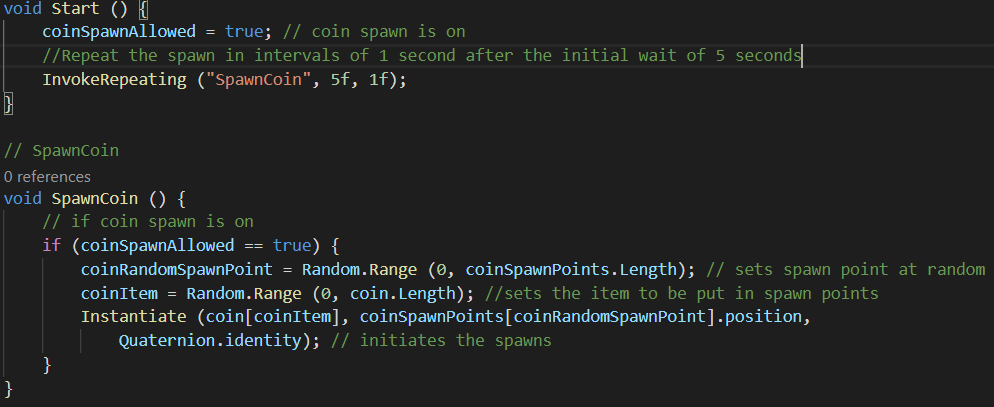
\includegraphics[width = 1\linewidth]{Images/CoinSpawn.PNG}
  \caption{Code snippet for CoinSpawn}
  \label{fig:CoinSpawn}
  \end{subfigure}
  \begin{subfigure}{.5\textwidth}
\centering
  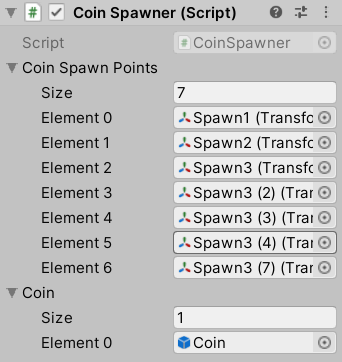
\includegraphics[width = 1\linewidth]{Images/CoinSpawnInspector.PNG}
  \caption{Coin spawn in the inspector}
  \label{fig:CoinSpawnInspect}
  \end{subfigure}
  \begin{subfigure}{.5\textwidth}
\centering
  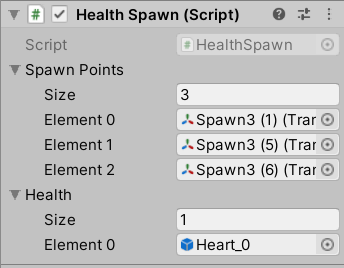
\includegraphics[width = 1\linewidth]{Images/HealthSpawnInspector.PNG}
  \caption{Health spawn in the inspector}
  \label{fig:HealthSpawnInspect}
    \end{subfigure}
  \end{figure}
  
  


